\section{Metoda bisekcji (połowienia)}
%%%%%%%%%%%%%%%%
\begin{frame}{Metoda bisekcji (połowienia)}
	\centering 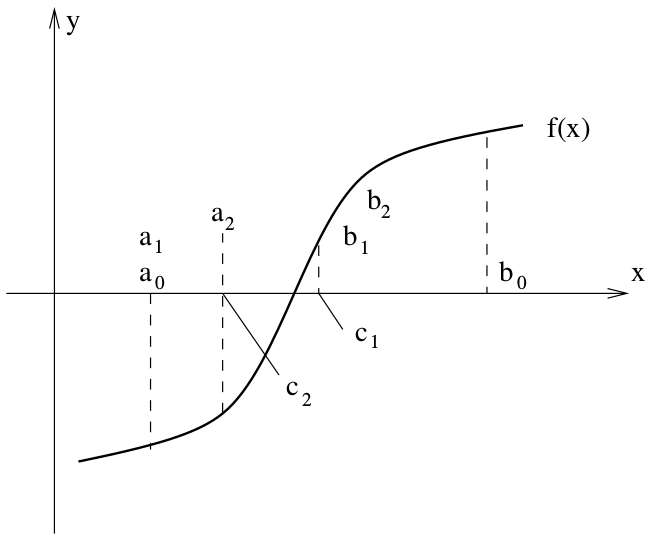
\includegraphics[width=.8\linewidth]{img/7/7_2_1}
\end{frame}
%%%%%%%%%%%%%%%%
\begin{frame}{Metoda bisekcji (połowienia)}
	\begin{table}[htbp]
		\begin{tabular}{|c|c|c|}
			\hline
			\multicolumn{1}{|c}{Dane:} & \multicolumn{2}{c|}{$a < b : \quad f(a) \cdot f(b) < 0$}\\
			\multicolumn{1}{|c}{} & \multicolumn{2}{c|}{$N$ - liczba iteracji (ustalona)}\\
			\multicolumn{1}{|c}{} & \multicolumn{2}{c|}{$d := b - a$}\\
			
			\hline
			
			\multicolumn{1}{|c}{\quad for} & \multicolumn{1}{c}{i := 1 to N do} & \text{}\\
			\cline{2-3}
			\multicolumn{1}{|c}{} & \multicolumn{2}{|c|}{c := (a + b) / 2}\\
			\cline{2-3}
			\multicolumn{1}{|c}{} & \multicolumn{2}{|c|}{f(c) $\cdot$ f(a)}\\
			\cline{2-3}
			\multicolumn{1}{|c|}{} & $<$ 0 & $>$ 0\\
			\multicolumn{1}{|c|}{} & b := c & a := c\\
			
			\hline
			
			\multicolumn{3}{|c|}{$\alpha$ := c}\\
			\multicolumn{3}{|c|}{E := d/$2^N$}\\
			\hline
		\end{tabular}
		\label{tab:transcap}
	\end{table}

	detekcja f(c) = 0\linebreak
	$\alpha$ : początkowo : w [$a_{0}$, $b_{0}$] $\rightarrow$ $b_{0}$ - $a_{0}$\linebreak
	\phantom{x} \hspace{0.2cm} po $N$ krokach : w [$a_{N}$, $b_{N}$] $\rightarrow$ błąd $\Rightarrow$
	\[
		E = b_{N} - a_{N} = \frac{b_{N-1} - a_{N-1}}{2} = \ldots = \frac{b_{0} - a_{0}}{2^{N}}
	\]
\end{frame}
%%%%%%%%%%%%%%%%
\begin{frame}{Metoda bisekcji (połowienia)}
	Charakterystyka:
	\begin{itemize}
		\item gwarancja zbieżności
		\item wolno zbieżna $\leftarrow$ wykorzystywana informacja: znak funkcji
		\item $>$ niż 1 zero $\rightarrow$ znajduje jedno z nich
		\item osobliwość $\rightarrow$ znajduje $\rightarrow$ ?
		\item kryterium zbieżności:
		\begin{itemize}
			\item $E \approx 10^{-6}$ $\rightarrow$ dobre dla $\lvert\alpha\rvert \sim 1$, złe $\rightarrow$ $\lvert\alpha\rvert \sim 10^{-26}$
			\item zwykle: $E = \epsilon \cdot \frac{a_{0} + b_{0}}{2}$ \quad $\epsilon$ - maszynowe!
			\item $\alpha \approx 0$ $\rightarrow$ specjalny przypadek
		\end{itemize}
	\end{itemize}
\end{frame}
